\documentclass{ximera}

\usepackage{epsfig}

\graphicspath{
  {./}
  {figures/}
}

\usepackage{epstopdf}
%\usepackage{ulem}
\usepackage[normalem]{ulem}

\epstopdfsetup{outdir=./}

\usepackage{morewrites}
\makeatletter
\newcommand\subfile[1]{%
\renewcommand{\input}[1]{}%
\begingroup\skip@preamble\otherinput{#1}\endgroup\par\vspace{\topsep}
\let\input\otherinput}
\makeatother

\newcommand{\EXER}{}
\newcommand{\includeexercises}{\EXER\directlua{dofile(kpse.find_file("exercises","lua"))}}

\newenvironment{computerExercise}{\begin{exercise}}{\end{exercise}}

%\newcounter{ccounter}
%\setcounter{ccounter}{1}
%\newcommand{\Chapter}[1]{\setcounter{chapter}{\arabic{ccounter}}\chapter{#1}\addtocounter{ccounter}{1}}

%\newcommand{\section}[1]{\section{#1}\setcounter{thm}{0}\setcounter{equation}{0}}

%\renewcommand{\theequation}{\arabic{chapter}.\arabic{section}.\arabic{equation}}
%\renewcommand{\thefigure}{\arabic{chapter}.\arabic{figure}}
%\renewcommand{\thetable}{\arabic{chapter}.\arabic{table}}

%\newcommand{\Sec}[2]{\section{#1}\markright{\arabic{ccounter}.\arabic{section}.#2}\setcounter{equation}{0}\setcounter{thm}{0}\setcounter{figure}{0}}
  
\newcommand{\Sec}[2]{\section{#1}}

\setcounter{secnumdepth}{2}
%\setcounter{secnumdepth}{1} 

%\newcounter{THM}
%\renewcommand{\theTHM}{\arabic{chapter}.\arabic{section}}

\newcommand{\trademark}{{R\!\!\!\!\!\bigcirc}}
%\newtheorem{exercise}{}

\newcommand{\dfield}{{\sf SlopeField}}

\newcommand{\pplane}{{\sf PhasePlane}}

\newcommand{\PPLANE}{{\sf PHASEPLANE}}

% BADBAD: \newcommand{\Bbb}{\bf}. % Package amsfonts Warning: Obsolete command \Bbb; \mathbb should be used instead.

\newcommand{\R}{\mbox{$\mathbb{R}$}}
\let\C\relax
\newcommand{\C}{\mbox{$\mathbb{C}$}}
\newcommand{\Z}{\mbox{$\mathbb{Z}$}}
\newcommand{\N}{\mbox{$\mathbb{N}$}}
\newcommand{\D}{\mbox{{\bf D}}}

\newcommand{\WW}{\mathcal{W}}

\usepackage{amssymb}
%\newcommand{\qed}{\hfill\mbox{\raggedright$\square$} \vspace{1ex}}
%\newcommand{\proof}{\noindent {\bf Proof:} \hspace{0.1in}}

\newcommand{\setmin}{\;\mbox{--}\;}
\newcommand{\Matlab}{{M\small{AT\-LAB}} }
\newcommand{\Matlabp}{{M\small{AT\-LAB}}}
\newcommand{\computer}{\Matlab Instructions}
\renewcommand{\computer}{M\small{ATLAB} Instructions}
\newcommand{\half}{\mbox{$\frac{1}{2}$}}
\newcommand{\compose}{\raisebox{.15ex}{\mbox{{\scriptsize$\circ$}}}}
\newcommand{\AND}{\quad\mbox{and}\quad}
\newcommand{\vect}[2]{\left(\begin{array}{c} #1_1 \\ \vdots \\
 #1_{#2}\end{array}\right)}
\newcommand{\mattwo}[4]{\left(\begin{array}{rr} #1 & #2\\ #3
&#4\end{array}\right)}
\newcommand{\mattwoc}[4]{\left(\begin{array}{cc} #1 & #2\\ #3
&#4\end{array}\right)}
\newcommand{\vectwo}[2]{\left(\begin{array}{r} #1 \\ #2\end{array}\right)}
\newcommand{\vectwoc}[2]{\left(\begin{array}{c} #1 \\ #2\end{array}\right)}

\newcommand{\ignore}[1]{}


\newcommand{\inv}{^{-1}}
\newcommand{\CC}{{\cal C}}
\newcommand{\CCone}{\CC^1}
\newcommand{\Span}{{\rm span}}
\newcommand{\rank}{{\rm rank}}
\newcommand{\trace}{{\rm tr}}
\newcommand{\RE}{{\rm Re}}
\newcommand{\IM}{{\rm Im}}
\newcommand{\nulls}{{\rm null\;space}}

\newcommand{\dps}{\displaystyle}
\newcommand{\arraystart}{\renewcommand{\arraystretch}{1.8}}
\newcommand{\arrayfinish}{\renewcommand{\arraystretch}{1.2}}
\newcommand{\Start}[1]{\vspace{0.08in}\noindent {\bf Section~\ref{#1}}}
\newcommand{\exer}[1]{\noindent {\bf \ref{#1}}}
\newcommand{\ans}{\textbf{Answer:} }
\newcommand{\matthree}[9]{\left(\begin{array}{rrr} #1 & #2 & #3 \\ #4 & #5 & #6
\\ #7 & #8 & #9\end{array}\right)}
\newcommand{\cvectwo}[2]{\left(\begin{array}{c} #1 \\ #2\end{array}\right)}
\newcommand{\cmatthree}[9]{\left(\begin{array}{ccc} #1 & #2 & #3 \\ #4 & #5 &
#6 \\ #7 & #8 & #9\end{array}\right)}
\newcommand{\vecthree}[3]{\left(\begin{array}{r} #1 \\ #2 \\
#3\end{array}\right)}
\newcommand{\cvecthree}[3]{\left(\begin{array}{c} #1 \\ #2 \\
#3\end{array}\right)}
\newcommand{\cmattwo}[4]{\left(\begin{array}{cc} #1 & #2\\ #3
&#4\end{array}\right)}

\newcommand{\Matrix}[1]{\ensuremath{\left(\begin{array}{rrrrrrrrrrrrrrrrrr} #1 \end{array}\right)}}

\newcommand{\Matrixc}[1]{\ensuremath{\left(\begin{array}{cccccccccccc} #1 \end{array}\right)}}



\renewcommand{\labelenumi}{\theenumi}
\newenvironment{enumeratea}%
{\begingroup
 \renewcommand{\theenumi}{\alph{enumi}}
 \renewcommand{\labelenumi}{(\theenumi)}
 \begin{enumerate}}
 {\end{enumerate}
 \endgroup}

\newcounter{help}
\renewcommand{\thehelp}{\thesection.\arabic{equation}}

%\newenvironment{equation*}%
%{\renewcommand\endequation{\eqno (\theequation)* $$}%
%   \begin{equation}}%
%   {\end{equation}\renewcommand\endequation{\eqno \@eqnnum
%$$\global\@ignoretrue}}

%\input{psfig.tex}

\author{Martin Golubitsky and Michael Dellnitz}

%\newenvironment{matlabEquation}%
%{\renewcommand\endequation{\eqno (\theequation*) $$}%
%   \begin{equation}}%
%   {\end{equation}\renewcommand\endequation{\eqno \@eqnnum
% $$\global\@ignoretrue}}

\newcommand{\soln}{\textbf{Solution:} }
\newcommand{\exercap}[1]{\centerline{Figure~\ref{#1}}}
\newcommand{\exercaptwo}[1]{\centerline{Figure~\ref{#1}a\hspace{2.1in}
Figure~\ref{#1}b}}
\newcommand{\exercapthree}[1]{\centerline{Figure~\ref{#1}a\hspace{1.2in}
Figure~\ref{#1}b\hspace{1.2in}Figure~\ref{#1}c}}
\newcommand{\para}{\hspace{0.4in}}

\usepackage{ifluatex}
\ifluatex
\ifcsname displaysolutions\endcsname%
\else
\renewenvironment{solution}{\suppress}{\endsuppress}
\fi
\else
\renewenvironment{solution}{}{}
\fi

\ifcsname answer\endcsname
\renewcommand{\answer}{}
\fi

%\ifxake
%\newenvironment{matlabEquation}{\begin{equation}}{\end{equation}}
%\else
\newenvironment{matlabEquation}%
{\let\oldtheequation\theequation\renewcommand{\theequation}{\oldtheequation*}\begin{equation}}%
  {\end{equation}\let\theequation\oldtheequation}
%\fi

\makeatother

\newcommand{\RED}[1]{{\color{red}{#1}}} 


\title{Discontinuous Forcing}

\begin{document}
\begin{abstract}
\end{abstract}
\maketitle

 \label{S:13.4}


In Section~\ref{S:resonance} we saw how to find solutions to a second 
order ordinary differential equation modeling the dynamics of a periodically
forced undamped spring\index{spring!undamped!periodically forced}.  
In particular, we studied equation \eqref{eq:uspf}, a variant of 
which is reproduced here:
\begin{equation}  \label{eq:ivH1}
\begin{array}{rcl}
   \ddot{x} + 4x & = & g(t) \\
    x(0) & = & 1 \\
    \dot{x}(0) & = & 0,
\end{array}
\end{equation}
where $g(t)=\cos(at)$.

We now assume that for a certain period of time there is no external 
force\index{external force}
acting on the spring and that, at some point, the situation changes. 
After that time the spring is subjected to an external forcing term.  
Specifically, we study the solution of \eqref{eq:ivH1} where $g(t)$ is 
assumed to have the simplest type of forcing with these properties, 
that is,  
\begin{equation}  \label{eq:Heavy1}
g(t) = H_1(t). 
\end{equation}
So until time $t=1$ there is no force on the spring, and after time $t=1$
there is a unit force acting on the spring.

The first step in solving the initial value problem \eqref{eq:ivH1} is to 
apply the Laplace transform to both sides of the equation to obtain:
\[
s^2{\cal L}[x]-s + 4{\cal L}[x] = {\cal L}[H_1] = \frac{1}{s}e^{-s}.
\]
Here we have used the initial conditions $x(0)=1$ and $\dot{x}(0)=0$.

In the second step we solve this equation for ${\cal L}[x]$ and obtain: 
\[
{\cal L}[x] = \frac{1}{s^2+4}\left( \frac{1}{s}e^{-s}+s\right)
=\frac{1}{s(s^2+4)}e^{-s}+\frac{s}{s^2+4}.
\]
This result is simplified by using partial fractions to obtain:
\[
\frac{1}{s(s^2+4)}=\frac{1}{4}\left(\frac{1}{s}-\frac{s}{s^2+4}\right).
\]
Therefore,
\[
{\cal L}[x] = \frac{1}{4}\left(\frac{1}{s}e^{-s}\right) -
\frac{1}{4}\frac{s}{s^2+4}e^{-s} + \frac{s}{s^2+4}.
\]

In the third step we use the inverse Laplace transform to solve for $x(t)$. 
In particular,
\[
x = \frac{1}{4}{\cal L}\inv\left[\frac{1}{s}e^{-s}\right] - 
\frac{1}{4}{\cal L}\inv\left[\frac{s}{s^2+4}e^{-s}\right] + 
{\cal L}\inv\left[\frac{s}{s^2+4}\right].
\]
Using Table~\ref{tab:Laplist} we obtain
\[
x(t) = \frac{1}{4}H_1(t) - 
\frac{1}{4}{\cal L}\inv\left[\frac{s}{s^2+4}e^{-s}\right](t) + \cos(2t).
\]
It remains to find the inverse Laplace transform of $\frac{s}{s^2+4}e^{-s}$.  
This calculation can be done using Proposition~\ref{prop:eHcLap2}, and we 
obtain
\begin{eqnarray*}
x(t) & = & \frac{1}{4}H_1(t) - \frac{1}{4}H_1(t)\cos(2(t-1)) + \cos(2t) \\
& = & \frac{1}{4}H_1(t)(1-\cos(2(t-1))) + \cos(2t).
\end{eqnarray*}
Note that the function 
\[
H_1(t)(1-\cos(2(t-1)))
\]
is differentiable, even though the step function $H_1(t)$ is discontinuous.
See Exercise~\ref{Ex:cont}.

\subsubsection*{An Example with Impulse Forcing}

We are now in a position to solve initial value problems having forcing 
functions that are impulse functions.   Indeed, as an example we solve
\begin{equation}  \label{eq:delta1}
\begin{array}{rcl}
\dot x + x & = & \delta_2(t)\\
x(0) & = & 1,
\end{array}
\end{equation}
using Laplace transforms.  Indeed, an application of ${\cal L}$ to
\eqref{eq:delta1} leads to
\[
s{\cal L}[x]-1 + {\cal L}[x] = e^{-2s},
\]
and therefore
\[
{\cal L}[x]=\frac{e^{-2s}+1}{s+1}=e^{-2s}\frac{1}{s+1}+\frac{1}{s+1}.
\]
Now we can use Proposition~\ref{prop:eHcLap2} combined with 
Table~\ref{tab:Laplist} to see that
\[
x(t) = {\cal L}^{-1}\left[e^{-2s}\frac{1}{s+1}\right](t)+ 
{\cal L}^{-1}\left[\frac{1}{s+1}\right](t) = 
H_2(t)e^{-(t-2)} + e^{-t}.
\]
Not surprisingly, this solution has a jump discontinuity at $t=2$ (see 
Figure~\ref{fig:delta1sol}); that is, the jump discontinuity occurs at 
the time when the impulse force is applied.
\begin{figure}[htb]
           \centerline{%
           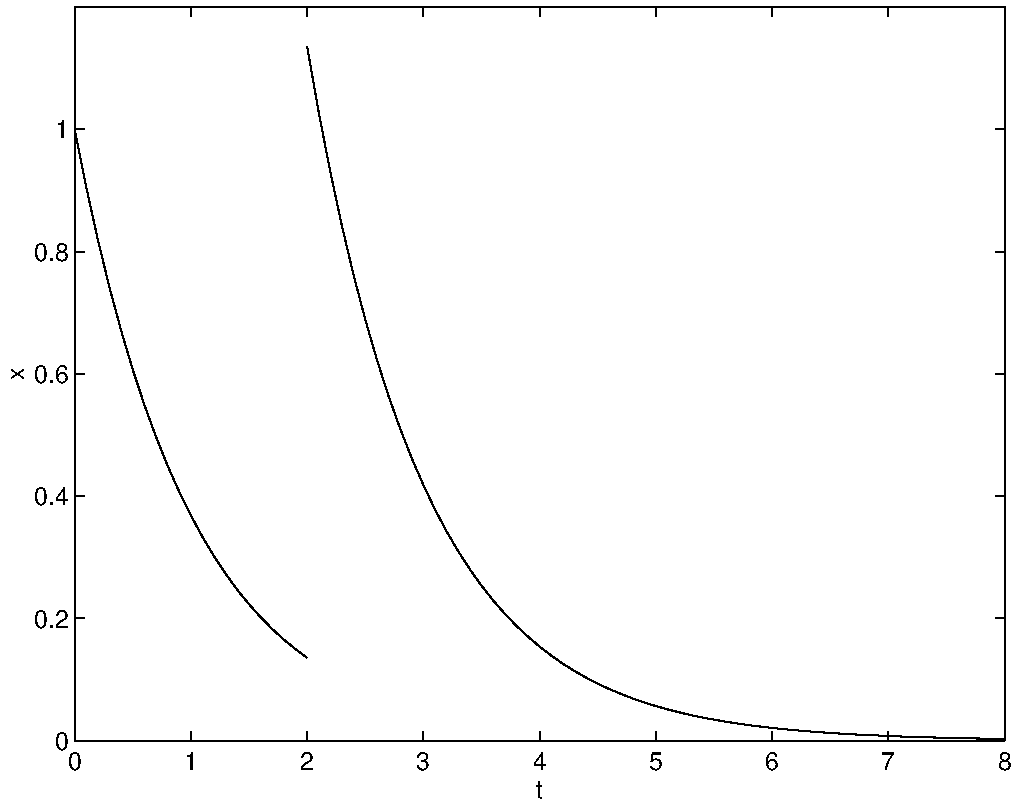
\includegraphics[width=2.8in]{../figures/d1sol.pdf}}
           \caption{The solution of the initial value problem
	   \protect\eqref{eq:delta1}.}
           \label{fig:delta1sol}
\end{figure}


\subsection*{Grand Finale}

We end this section by using Laplace transforms to solve the initial 
value problem:
\begin{equation}  \label{eq:lapendexam}
\begin{array}{rcl}
\ddot x + 4\dot x +5x  & = & \delta_1(t)+2H_3(t) \\
x(0) & = & 0 \\
\dot x(0) & = & 1.
\end{array}
\end{equation}
When solving \eqref{eq:lapendexam} we use most of the techniques that we have 
introduced so far.  

Applying the Laplace transform to both sides of the differential
equation in \eqref{eq:lapendexam} and using the initial conditions leads to
\[
s^2{\cal L}[x] -1 + 4s{\cal L}[x] + 5{\cal L}[x]=
e^{-s} +2\frac{e^{-3s}}{s}.
\]
Solving this equation for the Laplace transform of $x$ yields
\[
{\cal L}[x] = \frac{e^{-s} +2\frac{e^{-3s}}{s}+1}{s^2+4s+5}
= \frac{e^{-s}+1}{s^2+4s+5}+ \frac{2e^{-3s}}{s(s^2+4s+5)}.
\]

To find the inverse Laplace transform\index{Laplace transform!inverse}
of this equation, we need to 
compute the partial fraction expansion of 
\[
\frac{p(s)}{q(s)} = \frac{1}{s(s^2+4s+5)}.
\]
Defining {\tt p=[1]} and {\tt q=[1 4 5 0]} we use the 
command {\tt [c,r] = residue(p,q)}\index{\computer!residue} to obtain 
\begin{verbatim}
c =
  -0.1000 + 0.2000i
  -0.1000 - 0.2000i
   0.2000          
r =
  -2.0000 + 1.0000i
  -2.0000 - 1.0000i
        0          
\end{verbatim}

Hence the roots of $s^2+4s+5$ are $-2\pm i$, and we have
\[
\frac{1}{s(s^2+4s+5)} = \frac{-0.1 + 0.2i}{s-(-2+i)}+
\frac{-0.1-0.2i}{s-(-2-i)}+\frac{0.2}{s}.
\]
We combination the complex conjugate terms by typing
\begin{verbatim}
[num,denom] = realform(c(1),r(1))
\end{verbatim}\index{partial fractions!in \Matlab!{\tt realform}}
and obtain
\begin{verbatim}
num =
    -0.2000   -0.4000
denom =
     -2     1
\end{verbatim}
The partial fractions result is:
\[
\frac{1}{s(s^2+4s+5)} = -\frac{0.2(s+2)+0.4}{(s+2)^2+1}
+\frac{0.2}{s}.
\]

Now we can rewrite ${\cal L}[x]$ as
\begin{eqnarray*}
{\cal L}[x] &=& \frac{e^{-s}}{(s+2)^2+1}+ \frac{1}{(s+2)^2+1}\\
&& +2e^{-3s}\left(-0.2\frac{s+2}{(s+2)^2+1}-0.4\frac{1}{(s+2)^2+1}
+0.2\frac{1}{s}\right).
\end{eqnarray*}
We use Proposition~\ref{prop:eHcLap1}(a) to see that
\begin{eqnarray*}
{\cal L}\inv\left[\frac{1}{(s+2)^2+1}\right]&=&
e^{-2t}\sin(t)\\
{\cal L}^{-1}\left[\frac{s+2}{(s+2)^2+1}\right]&=&
e^{-2t}\cos(t),
\end{eqnarray*}
and Proposition~\ref{prop:eHcLap2}(b) to see that
\begin{eqnarray*}
{\cal L}^{-1}\left[e^{-s}\frac{1}{(s+2)^2+1}\right]&=&
H_1(t)e^{-2(t-1)}\sin(t-1)\\
{\cal L}^{-1}\left[e^{-3s}\frac{s+2}{(s+2)^2+1}\right]&=&
H_3(t)e^{-2(t-3)}\cos(t-3)\\
{\cal L}^{-1}\left[e^{-3s}\frac{1}{(s+2)^2+1}\right]&=&
H_3(t)e^{-2(t-3)}\sin(t-3).
\end{eqnarray*}
Now we can write down the solution $x(t)$ as
\begin{eqnarray*}
x(t) &=& H_1(t)e^{-2(t-1)}\sin(t-1)+e^{-2t}\sin(t)\\
&&-0.4 H_3(t)e^{-2(t-3)}\cos(t-3) -0.8 H_3(t)e^{-2(t-3)}\sin(t-3)
+0.4 H_3(t)\\
&=& H_1(t)e^{-2(t-1)}\sin(t-1)+e^{-2t}\sin(t)\\
&& -0.4 H_3(t)e^{-2(t-3)}(\cos(t-3)+2\sin(t-3))+0.4 H_3(t).
\end{eqnarray*}
The solution is shown in Figure~\ref{fig:lapallsol}.
The two changes in the behavior of the solution occurring at 
$t=1$ and at $t=3$ are readily observed.  
\begin{figure}[htb]
           \centerline{%
           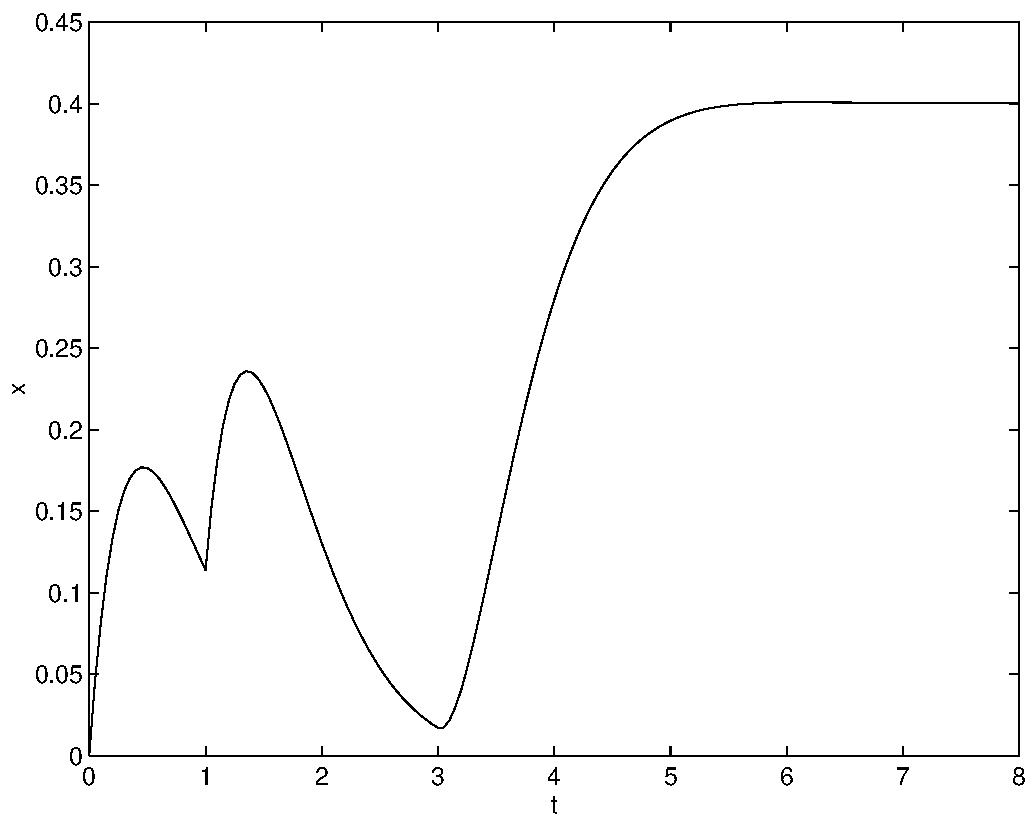
\includegraphics[width=3.2in]{../figures/dallsol.pdf}}
           \caption{The solution of the initial value problem
           \protect\eqref{eq:lapendexam}.}
           \label{fig:lapallsol}
\end{figure}

Note that the solution to \eqref{eq:lapendexam} tends asymptotically to 
$x=0.4$  for large $t$.  This behavior can be explained as follows.  For large 
$t$, equation \eqref{eq:lapendexam} becomes
\[
\ddot x + 4\dot x +5x = 2.
\]
The only equilibrium (or time independent solution) to this equation is
$x(t)=0.4$, and each solution of \eqref{eq:lapendexam} tends to that equilibrium 
for large $t$.




\includeexercises


\end{document}
